% !Mode:: "TeX:UTF-8"
% Author: Zhengxi Tian
% Email: zhengxi.tian@hotmail.com

\chapter{研究方法}\label{ch:method}

% -- 简要说明实验框架。并不复杂,一图足矣。
% 详细说明数据集的统计数据,模型的超参数,训练参数,指标实现的来源,
% 指标的超参数。这些属于Training Procedure或者Experiment的内容。
% 因为是本科毕设,写verbose一些也没关系。
\section{指标测评框架}\label{sec:eval_framework}
我们的实验主要涉及在多个数据集上训练多个模型,然后用多种指标去测量这些系统的句子层面得分和系统层面得分。
表~\ref{tab:experiment_triples}~展示了实验所使用的模型,数据集和指标。
% -- Math & Figure
如图~\ref{fig:framework}~所示,我们的实验首先从对每一个模型$m$和数据集$d$的组合$(m, d) \in M \times D$在训练集上进行训练,
并让训练好的$(m, d)$在测试集上解码产生响应$r$,然后再用每一个指标$s \in S$去给$r$在句子层面和系统层面上打分,分别得到$\lambda_{u}$和$\lambda_{s}$。实验的最终结果是获得一个5元组$(m, d, e, \lambda_{u}, \lambda_{s})$,表示在数据集$d$上训练的模型$m$在指标$s$的评价下所得的句子层面得分$\lambda_u$和系统层面得分$\lambda_s$。


%本章将详细介绍模型的超参数,训练流程,数据集预处理等实验细节。
\begin{table}[H]
    \centering
    \caption{实验对象一览}
    \label{tab:experiment_triples}
    \begin{tabular}{|r|m{0.6\textwidth}|}
        \hline
        模型 & HRED,LSTM,VHRED \\
        \hline
        数据集 & Ubuntu,OpenSubtitles,LSDSCC \\
        \hline
        指标 & BLEU,ROUGE,METEOR,Vector-Average,
        Vector-Extrema,Greedy-Matching,
        ADEM,PPL,Distinct-N \\
        \hline
    \end{tabular}
\end{table}

\begin{figure}[H]
    \centering
    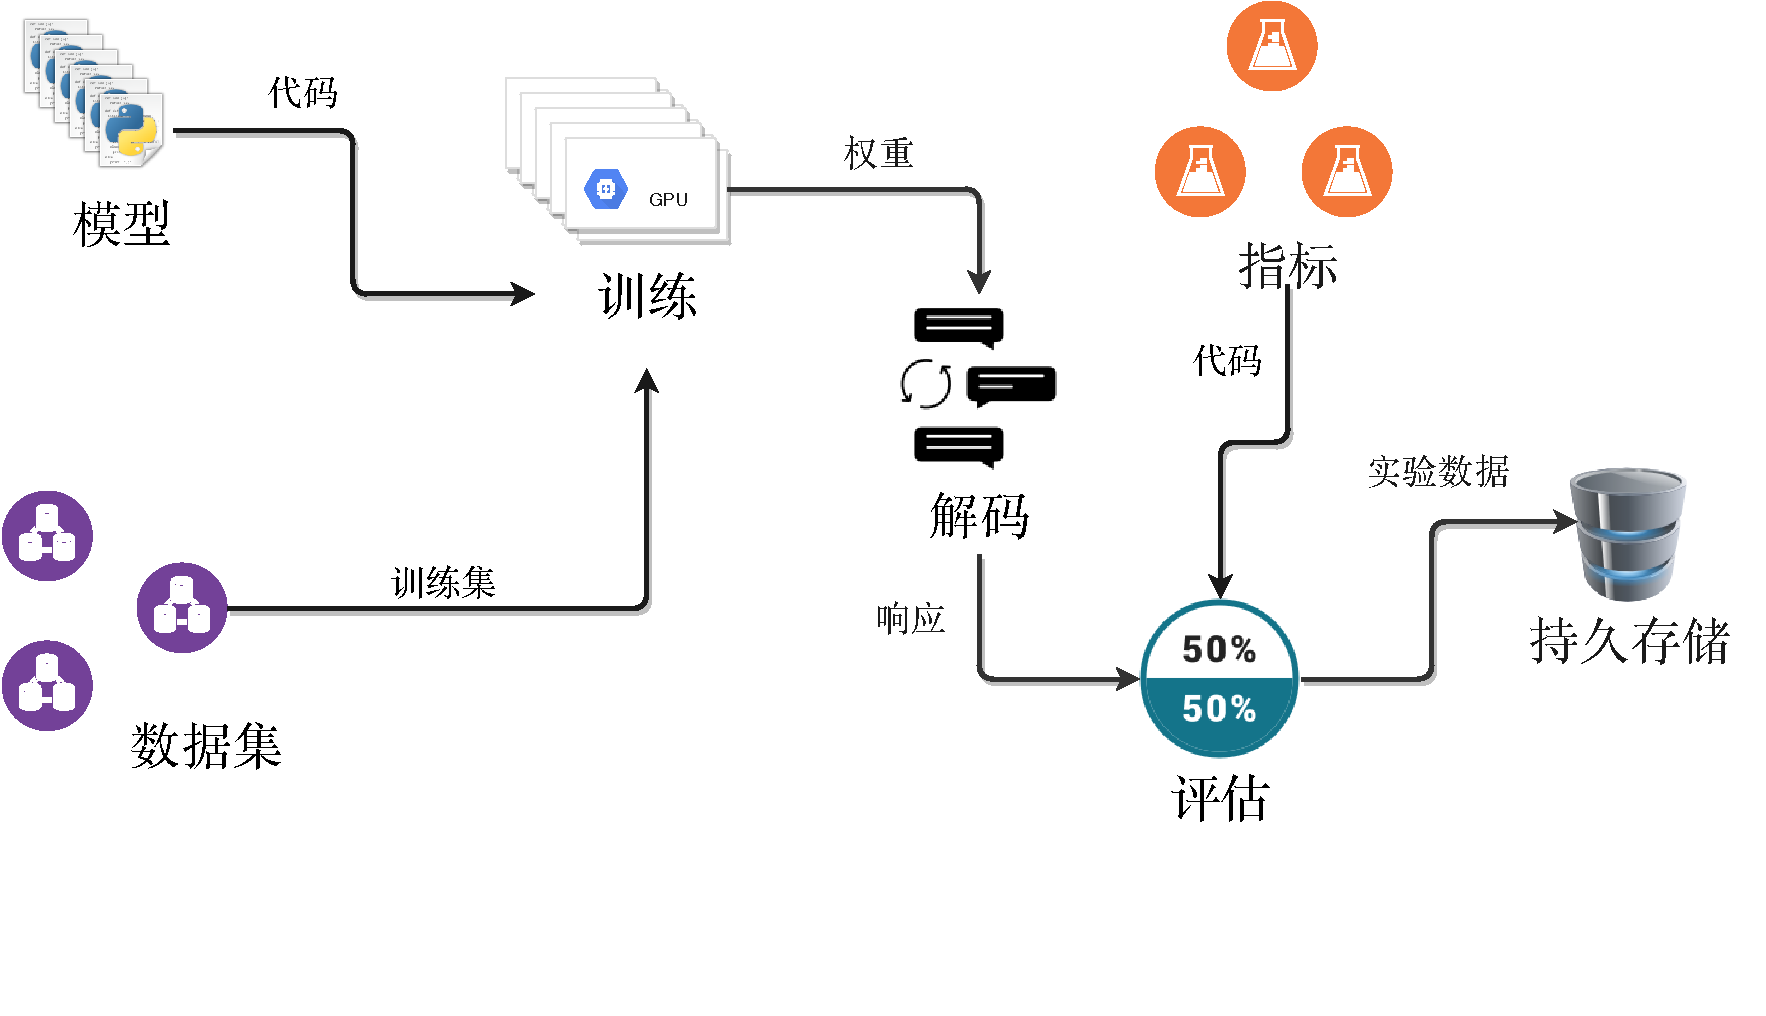
\includegraphics[width=0.8\textwidth]{figure/drawio/eval_v3.pdf}
    \caption{实验框架}
    \label{fig:framework}
\end{figure}

\section{模型超参数设置}\label{sec:model_hparams}
% ------ Model setup ----------- %
在模型超参数方面,我们的设置大致和\cite{VHRED}相同。
我们用Adam\upcite{AdamOpt}来优化所有模型,
batch\_size统一设为20。
% -- Dimension of Word Embeddings -- %
我们在Ubuntu上使用维度是300的词嵌入,
在OpenSubtitles和LSDSCC上使用维度是400的词嵌入。
% -- Hidden Units of Utterance Encoder -- %
HRED和VHRED的句子编码器(Utterance Encoder)
在Ubuntu上使用500个隐藏单元,
在OpenSubtitles和LSDSCC上使用1000个隐藏单元
\footnote{这里的LSTM模型是一个语言模型,所以它既没有编码RNN,
也没有上下文RNN,只有解码RNN。}。
% -- Hidden Units of Context Encoder -- %
HRED和VHRED的上下文编码器(Context Encoder)
在所有数据集上都使用1000个隐藏单元。
% -- Hidden Units of Utterance Decoder -- %
不同模型的句子解码器(Utterance Decoder)
在不同数据集上各有不同,
如表~\ref{tab:utterance_decoder_hidden_units}~所示。
我们根据数据集的特点来设置不同RNN的隐藏单元数目,
通常在样本数多或者词汇表大的数据集上训练时,
模型的隐藏单元数目会更多。

\begin{table}[H]
    \centering
    \caption{句子解码器的隐层状态单元数目}
    \label{tab:utterance_decoder_hidden_units}
    \begin{tabular}{llll}
        \toprule
        & HRED & LSTM & VHRED \\
        \midrule
        LSDSCC & 1000 & 2000 & 1000 \\
        OpenSubtitles & 1000 & 2000 & 1000 \\
        Ubuntu & 500 & 2000 & 500 \\
        \bottomrule
    \end{tabular}
\end{table}

% -- Direction of Utterance Encoder -- %
Ubuntu上的模型的句子编码器都使用了单向RNN,
而OpenSubtitles和LSDSCC上的模型的句子编码器则使用双向RNN。
% -- Gate Type of Utterance & Context Encoder -- %
所有模型的句子编码器和上下文编码器(如果有)都使用GRU作为门单元。
% -- Gate Type of Decoder -- %
句子解码器的门单元类型如表~\ref{tab:utterance_decoder_gate_types}~所示
\footnote{由于失误,OpenSubtitles和LSDSCC上的LSTM模型的解码器都没有使用LSTM门单元,不过它们仍然是语言模型。}。
\begin{table}[H]
    \centering
    \caption{句子解码器的门单元类型}
    \label{tab:utterance_decoder_gate_types}
    \begin{tabular}{llll}
        \toprule
        & HRED & LSTM & VHRED \\
        \midrule
        LSDSCC & LSTM & GRU & GRU \\
        OpenSubtitles & LSTM & GRU & GRU \\
        Ubuntu & LSTM & LSTM & LSTM \\
        \bottomrule
    \end{tabular}
\end{table}

所有的模型都在一台GeForce GTX TITAN X上训练了至少1周。
模型收敛时的困惑度如表~\ref{tab:converged_perplexity}~所示。
\begin{table}[H]
    \centering
    \caption{}
    \label{tab:converged_perplexity}
    \begin{tabular}{llll}
        \toprule
        & HRED & LSTM & VHRED \\
        \midrule
        LSDSCC & & &  \\
        OpenSubtitles & & &  \\
        Ubuntu & & &  \\
        \bottomrule
    \end{tabular}
\end{table}

与\cite{VHRED}不同的是,我们没有用预训练的HRED的参数来初始化对应的VHRED。
从实验结果来看,从零开始训练的VHRED也能达到和HRED相匹配的性能。
所有的模型都使用了梯度剪裁,阈值为1。
所有模型在Ubuntu上的学习率为0.0002,
在OpenSubtitles和LSDSCC上的学习率为0.0001。
在解码时,我们使用随机取样。

\section{数据集预处理及其统计数据}
\label{sec:dataset_proprecessing}

\section{指标配置}\label{sec:metric_config}

\section{本章小结}\label{sec:method_conclusion}
